\subsection{Motivation}

As previously pointed out, the computation of quantities such as Yukawa couplings involves correlators of excited spin and twist fields.
After the analysis of the main contribution to amplitudes involving twist fields at the intersection of D-branes, we focus on the computation of correlators of (excited) spin fields.
This has been a research subject for many years until the formulation found in the seminal paper by Friedan, Martinec and Shenker~\cite{Friedan:1986:ConformalInvarianceSupersymmetry} based on bosonization.
In general the available techniques allow to compute only correlators involving ``Abelian'' configurations, that is configurations which can be factorized in sub-configurations having \U{1} symmetry.
Non Abelian cases have been considered~\cite{Inoue:1987:NonAbelianOrbifolds,Inoue:1990:StringInteractionsNonAbelian,Gato:1990:VertexOperatorsNonabelian,Frampton:2001:ClassificationConformalityModels,Pesando:2016:FullyStringyComputation} which is mathematically by far more complicated.
  
Despite the existence of an efficient method based on bosonization~\cite{Friedan:1986:ConformalInvarianceSupersymmetry} and old methods based on the Reggeon vertex~\cite{Sciuto:1969:GeneralVertexFunction,DellaSelva:1970:SimpleExpressionSciuto,Schwarz:1973:EvaluationDualFermion,DiVecchia:1990:VertexIncludingEmission,Nilsson:1990:GeneralNSRString,DiBartolomeo:1990:GeneralPropertiesVertices,Engberg:1993:AlgorithmComputingFourRamond,Petersen:1989:CovariantSuperreggeonCalculus}, we take into examination the computation of spin field correlators and propose a new method to compute them.
We hope to be able to extend this approach to correlators involving twist fields and non Abelian spin and twist fields.
We would also like to investigate the reason of the non existence of an approach equivalent to bosonization for twist fields.
At the same time we are interested to explore what happens to a CFT in presence of defects.
It turns out that, despite the defects, it is still possible to define a radial time dependent stress-energy tensor which satisfies the canonical OPE.
Moreover the boundary changing defects in the construction can be associated with excited spin fields enabling the computation of correlators involving excited spin fields without resorting to bosonization.



\subsection{Point-like Defect CFT: the Minkowskian Formulation}
\label{sec:Mink_theory}
  
Let $( \tau,\, \sigma ) \in \Sigma = ( -\infty,\, +\infty) \times \qty[ 0, \pi ]$ define a strip with Lorentzian metric and consider $N_f$ massless complex fermions $\psi^i$ such that $i = 1,\, 2,\, \dots,\, N_f$.
Their two-dimensional Minkowski action defined on the strip $\Sigma$ is:
\begin{equation}
  S
  =
  \frac{T}{2}
  \infinfint{\tau}
  \finiteint{\sigma}{0}{\pi}
  \qty(
    \frac{1}{2}\, \bpsi_i( \tau,\, \sigma )\,
    \qty( -i \gamma^{\alpha} \lrpartial{\alpha} )\,
    \psi^i( \tau,\, \sigma ) 
  ),
  \label{eq:cft-action_full}
\end{equation}
where the gamma matrices are
\begin{equation}
  \gamma^{\tau}
  =
  \mqty( & 1 \\ -1 & )
  =
  -\gamma_{\tau},
  \qquad
  \gamma^{\sigma}
  =
  \mqty( & 1 \\ 1 & )
  =
  \gamma_{\sigma},
\end{equation}
and the components of the massless fermions are
\begin{equation}
  \psi
  =
  \mqty( \psi_+ \\ \psi_- ),
  \qquad
  \bpsi
  =
  \psi^{\dagger}\, \gamma^{\tau}
  =
  \mqty( -\psi_-^* & \psi_+^* ).
\end{equation}
We then define the lightcone coordinates $\xi_{\pm} = \tau \pm \sigma$ such that $\ipd{\pm} = \frac{1}{2}\, \qty( \ipd{\tau} \pm \ipd{\sigma} )$.
In components the action reads:
\begin{equation}
  S
  =
  i \frac{T}{4}
  \infinfint{\xi_+}
  \infinfint{\xi_-}
  \qty(
    \psi^*_{-,\, i} \lrpartial{+} \psi^i_- + \psi^*_{+,\, i} \lrpartial{-} \psi^i_+
  ),
  \label{eq:cft-action}
\end{equation}
so the \eom are:
\begin{equation}
  \begin{split}
    \ipd{-} \psi_{+}^i( \xi_+, \xi_- )
    & =
    \ipd{+} \psi_{-}^i( \xi_+, \xi_- )
    =
    0,
    \\
    \ipd{-} \psi^*_{+,\, i}( \xi_+, \xi_- )
    & =
    \ipd{+} \psi^*_{-,\, i}( \xi_+, \xi_- )
    =
    0.
  \end{split}
  \label{eq:eom}
\end{equation}
Their solutions are the ``holomorphic'' functions $\psi_{+}^i(\xi_+)$ and $\psi_{-}^i(\xi_-)$ and their complex conjugates.\footnotemark{}
\footnotetext{%
  Notice that $\psi^*$ is indeed the complex conjugate of the field $\psi$, while it will no longer be the case in the Euclidean formalism.
}
\begin{figure}[tbp]
  \centering
  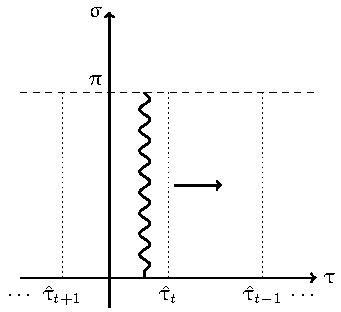
\includegraphics[width=0.4\linewidth]{img/point-like-defects}
  \caption{Propagation of the string in the presence of the worldsheet defects.}
  \label{fig:point-like-defects}
\end{figure}
The boundary conditions are instead:
\begin{equation}
  \eval{
    \qty(
      \var{\psi}_{+,\, i}^* \psi_{+}^{ i} +
      \var{\psi}_{-,\, i}^* \psi_{-}^{ i} -
      \psi_{+,\, i}^* \var{\psi}_{+}^{ i} -
      \psi_{-,\, i}^* \var{\psi}_{-}^{ i}
    )
  }_{\sigma = 0}^{\sigma = \pi} = 0.
  \label{eq:boundary-conditions}
\end{equation}
We solve the constraint imposing the non trivial relations:
\begin{equation}
  \begin{cases}
    \psi_-^i( \tau, 0 )
    =
    \tensor{\qty( R_{(t)} )}{^i_j}
    \psi^j_+( \tau, 0 ),
    & \qquad
    \tau \in \qty( \htau_{(t)}, \htau_{(t-1)} ),
    \\
    \psi_-^i( \tau, \pi )
    =
    - \psi_+^i( \tau, \pi ),
    & \qquad
    \tau \in \R,
  \end{cases}
  \label{eq:boundary-conditions-solutions}
\end{equation}
where $t = 1, 2, \dots, N$.
This way we introduce $N$ zero-dimensional defects on the boundary, pictorially shown in~\Cref{fig:point-like-defects}.
They are located on the strip at $( \htau_{(t)}, 0 ) \in \Sigma$ such that $\htau_{(t)} < \htau_{(t-1)}$ with $\htau_{N+1} = -\infty$ and $\htau_0 = +\infty$.
Their characterisation is given by $N$ matrices $R_{(t)} \in \U{N_f}$.
    
In most of this paper we want the in- and out-vacua to be the usual NS vacuum.
We thus choose the boundary condition at $\sigma = \pi$ so that when there are no defects the system describes NS fermions.
We require also the cancellation of the action of the defects at $\htau = \pm\infty$, that is:
\begin{equation}
  R_{(N)} R_{(N-1)} \dots R_{(1)} = \1.
\end{equation}
More general cases where the asymptotic vacua are twisted can be worked out in similar fashion.
   
In order to connect to the Euclidean formulation we introduce $N_f$ ``double fields'' $\Psi^i$.\footnotemark{}
\footnotetext{%
  In this case they correspond to the fields $\psi^i_+$.
}
They can be obtained by gluing $\psi^i_+$ and $\psi^i_-$ along the $\sigma = \pi$ boundary and labeled by an index $i = 1,\, 2,\, \dots,\, N_f$:
\begin{equation}
  \Psi^i(\tau,\, \phi)
  =
  \begin{cases}
    \psi^i_+(\tau,\, \phi),
    & \qquad 0\le\phi\le \pi
    \\
    -\psi^i_-(\tau,\, 2\pi-\phi),
    & \qquad \pi \le \phi \le 2 \pi        
  \end{cases}
  \label{eq:double-field-Lorentzian}
\end{equation}
where $0 \le \phi \le 2 \pi$.
The boundary conditions become:
\begin{equation}
  \Psi^i(\tau, 2 \pi )
  =
  - \tensor{\qty( R_{(t)} )}{^i_j}
  \Psi^j(\tau,\, 0 ),
  \qquad
  \tau \in \qty( \htau_{(t)},\, \htau_{(t-1)} ).
\end{equation}
Using the equation of motion we get $\Psi^i(\tau,\, \phi) = \Psi^i(\tau + \phi)$ and the boundary conditions become the (pseudo-)periodicity conditions
\begin{equation}
  \Psi^i(\tau + 2 \pi )
  =
  - \tensor{\qty( R_{(t)} )}{^i_j}
  \Psi^j(\tau ),
  \qquad
  \tau \in \qty( \htau_{(t)}, \htau_{(t-1)} ).
\end{equation}
The main issue is now to expand $\Psi$ in a basis of modes and proceed to its quantization.
Even in the simplest case $N_f = 1$ the task of finding the Minkowskian modes turns out to be fairly complicated.
It is however possible to overcome the issue in the Euclidean formalism.


\subsection{Conserved Product and Charges}
\label{sec:product}

In order to promote the theory to its quantum formulation, we define a procedure to build a Fock space of states in the Heisenberg formalism.
Equal time anti-commutation relations must then be invariant in time.
We thus need a time independent internal product to extract the creation and annihilation operators and expand the fields on the basis of modes.


\subsubsection{Conserved Product and Current}

Start from a generic conserved current
\begin{equation}
  j( \tau,\, \sigma )
  =
  j_{\tau}( \tau,\, \sigma )\, \dd{\tau} + j_{\sigma}( \tau,\, \sigma )\, \dd{\sigma},
\end{equation}
and consider
\begin{equation}
  \star j
  =
  j_{\sigma} \dd{\tau} + j_{\tau} \dd{\sigma}
  \quad
  \Rightarrow
  \quad
  \dd{(\star j)}
  =
  \qty( \ipd{\tau} j_{\tau} - \ipd{\sigma} j_{\sigma} ) \dd{\tau} \dd{\sigma},
\end{equation}
where $\star$ is the Hodge dual operator.
Integration over the surface $\Sigma' = [ \tau_i, \tau_f ] \times [ 0, \pi ]$ yields:
\begin{equation}
  \int\limits_{\Sigma'} \dd{(\star j)}
  =
  \int\limits_{\partial \Sigma'}
  \star j
  =
  0
  \qquad
  \Leftrightarrow
  \qquad
  \finiteint{\sigma}{0}{\pi}
  \eval{j_{\tau}}_{\tau = \tau_f}^{\tau = \tau_i}
  =
  \finiteint{\tau}{\tau_i}{\tau_f}
  \eval{j_{\sigma}}_{\sigma = \pi}^{\sigma = 0}.
\end{equation}
The current $j_{\tau}( \tau,\, \sigma )$ is thus conserved in time if
\begin{equation}
  \finiteint{\tau}{\tau_i}{\tau_f}
  \qty( \eval{j_{\sigma}}_{\sigma = \pi} - \eval{j_{\sigma}}_{\sigma = 0} )
  =
  0.
  \label{eq:time-conservation}
\end{equation}
In this case we can define
\begin{equation}
  Q = \finiteint{\sigma}{0}{\pi} j_{\tau}( \tau,\, \sigma ) 
\end{equation}
as conserved quantity (that is $\ipd{\tau} Q = 0$).
We now consider explicitly the symmetries of the action~\eqref{eq:cft-action}.
We focus on diffeomorphism invariance and $\U{N_f}$ flavour symmetries of the bulk theory leading to the stress-energy tensor and a vector current.


\subsubsection{Flavour Vector Current}

Consider first the $\U{N_f}$ vector current of the flavour symmetry in~\eqref{eq:cft-action_full}.
We write it as
\begin{equation}
  j_{\alpha}^a ( \tau,\, \sigma )
  =
  \tensor{\qty( \rT^a )}{^i_j}\,
  \bpsi_i( \tau,\, \sigma )\, \gamma_{\alpha}\, \psi^j( \tau,\, \sigma ),
\end{equation}
where $\rT^a$ is a generator of $\U{N_f}$ such that $a = 1,\, 2,\, \dots,\, N_f^2$.\footnotemark{}
\footnotetext{%
  The results however are more general and hold for a generic matrix $M$ taking the place of any of the generators $\rT^a$.
  Spinors $\psi$ and $\bpsi$ can also be generalized to two different and arbitrary solutions of the \eom~\eqref{eq:eom} while keeping the current conserved.
}
In components we have:
\begin{eqnarray}
  j^a_{\tau}( \tau,\, \sigma )
  & = &
  \tensor{\qty( \rT^a )}{^i_j}\,
  \qty( \psi^*_{+,\, i} \psi^j_+ + \psi^*_{-,\, i} \psi^j_- )
  \\
  j^a_{\sigma}( \tau,\, \sigma )
  & = &
  \tensor{\qty( \rT^a )}{^i_j}\,
  \qty( \psi^*_{+,\, i} \psi^j_+ - \psi^*_{-,\, i} \psi^j_- ).
\end{eqnarray}

In order to define a conserved charge, we require:
\begin{equation}
  \finiteint{\tau}{\tau_i}{\tau_f}
  \qty(
    \eval{j_{\sigma}^a}_{\sigma = \pi} - \eval{j_{\sigma}^a}_{\sigma = 0}
  )
  =
  0,
\end{equation}
where
\begin{equation}
  \eval{j_{\sigma}^a( \tau,\, \sigma )}_{\sigma = \pi} \equiv 0
\end{equation}
using the boundary conditions~\eqref{eq:boundary-conditions}.
Moreover we have:
\begin{equation}
  \eval{j_{\sigma}^a( \tau,\, \sigma )}_{\sigma = 0}
  =
  \qty[
    \psi^*_+\,
    \qty( \rT^a - R_{(t)}^{\dagger} \rT^a R_{(t)} )\,
    \psi_+
  ]_{\sigma = 0},
  \qquad
  \tau \in \qty( \htau_{(t)}, \htau_{(t-1)} ).
\end{equation}
In general
\begin{equation}
  \eval{j_{\sigma}^a( \tau,\, \sigma )}_{\sigma = 0}
  =
  0
  \qquad
  \Leftrightarrow
  \quad
  \rT^a \propto \1
\end{equation}
so that $R_{(t)}^{\dagger} \rT^a = \rT^a R_{(t)}^{\dagger}$.
This shows that the presence of the point-like defects on the worldsheet breaks the $\U{N_f}$ symmetry down to a \U{1} phase.\footnotemark{}
\footnotetext{%
  The symmetry is $\SO{N_f} \times \SO{N_f}$ if we consider Majorana-Weyl fermions.
}
The \U{1} vector current then defines a conserved charge for a restricted class of functions.

Let $\alpha$ and $\beta$ be two arbitrary (bosonic) solutions to the \eom~\eqref{eq:eom}, we define a product
\begin{equation}
  \consprod{\alpha}{\beta}
  =
  \cN
  \finiteint{\sigma}{0}{\pi}
  \qty( \alpha_{+,\, i}^* \beta_+^i + \alpha_{-,\, i}^* \beta_-^i ),
  \label{eq:conserved-product}
\end{equation}
where $\cN \in \R$ is a normalisation constant and the integrand must not present non integrable singularities.
The product is such that $\consprod{\alpha}{\beta} = \consprod{\alpha}{\beta}^*$.
We can also rewrite the result to the double fields defined in~\eqref{eq:double-field-Lorentzian}.
Let in fact $A$ and $B$ be the ``double
fields'' corresponding to $\alpha$ and $\beta$ respectively:
\begin{equation}
  \consprod{\alpha}{\beta}
  =
  \cN
  \finiteint{\phi}{0}{2\pi}\,
  A_i^*( \tau + \phi )\, B^i( \tau + \phi ).
  \label{eq:conserved-product-double-field}
\end{equation}

\subsubsection{Stress-Energy Tensor}

Consider the stress-energy tensor of the bulk theory.
Using the usual Nöther's procedure we get the on-shell non vanishing components:
\begin{equation}
  \begin{split}
    \cT_{++}( \xi_+ )
    & =
    -i \frac{T}{4} \psi_{+,\, i}^*( \xi_+ ) \lrpartial{+} \psi_+^i( \xi_+ ),
    \\
    \cT_{--}( \xi_- )
    & =
    -i \frac{T}{4} \psi_{-,\, i}^*( \xi_- )\lrpartial{-} \psi_-^i( \xi_- ).
  \end{split}
  \label{eq:stress-energy-tensor-lightcone}
\end{equation}
As always the boundary of $\Sigma$ breaks the symmetry for translations in the $\sigma$ direction, while the defects break the time translations: the Hamiltonian is therefore time-dependent but it is constant between two consecutive point-like defects.
In fact, from the definition of the stress-energy tensor, we can in principle
build the hypothetical charges:
\begin{eqnarray}
  \rH( \tau )
  & = &
  \finiteint{\sigma}{0}{\pi}
  \cT_{\tau\tau}( \tau,\, \sigma )
  =
  \finiteint{\sigma}{0}{\pi}
  \qty( \cT_{++}( \tau + \sigma ) + \cT_{--}( \tau - \sigma ) ),
  \label{eq:hamiltonian}
  \\
  \rP( \tau )
  & = &
  \finiteint{\sigma}{0}{\pi}
  \cT_{\tau\sigma}( \tau,\, \sigma )
  =
  \finiteint{\sigma}{0}{\pi}
  \qty( \cT_{++}( \tau + \sigma ) - \cT_{--}( \tau - \sigma ) ),
  \label{eq:momentum}
\end{eqnarray}
which are conserved if~\eqref{eq:time-conservation} holds.

We order the point-like defects as $\htau_{(t_0 - 1)} < \tau_i \le \htau_{(t_0)} < \htau_{(t_N)} \le \tau_f < \htau_{(t_N+1)}$.
For the linear momentum $\rP$ the condition of conservation
reads:\footnotemark{}
\footnotetext{%
  Notice that in the second term of the second line the differentiation with respect to $\tau$ is acting only on $R_{(t)}$ and $R_{(t)}^{\dagger}$.
}
\begin{equation}
  \begin{split}
    & \finiteint{\tau}{\tau_i}{\tau_f}
    \eval{\qty( \cT_{++}( \tau + \sigma ) + \cT_{--}( \tau - \sigma ) )}_{\sigma = 0}^{\sigma = \pi}
    \\
    & =
    - i \frac{T}{4}
    \int \Delta\tau
    \qty(
      2 \eval{\psi_{+,\, i}^*\, \lrpartial{\tau} \psi_+^i}^{\sigma = \pi}_{\sigma = 0}
      -
      \eval{\psi_{+,\, i}^* \tensor{\qty( R_{(t)}^{\dagger} \lrpartial{\tau} R_{(t)} )}{^i_j} \psi_+^j}_{\sigma = 0}
    )
    \neq
    0.
  \end{split}
\end{equation}
The corresponding condition for the Hamiltonian $\rH$ is:
\begin{equation}
  \begin{split}
    & \finiteint{\tau}{\tau_i}{\tau_f}
    \eval{\qty( \cT_{++}( \tau + \sigma ) - \cT_{--}( \tau - \sigma ) )}_{\sigma = 0}^{\sigma = \pi}
    \\
    & =
    - i \frac{T}{4}
    \int \Delta\tau
    \qty( \eval{\psi_{+,\, i}^* \tensor{\qty( R_{(t)}^{\dagger} \lrpartial{\tau} R_{(t)} )}{^i_j} \psi_+^j}_{\sigma = 0} )
    = 0
    \quad
    \Leftrightarrow
    \quad
    \qty( \tau_i, \tau_f ) \in \qty( \htau_{(t)}, \htau_{(t-1)} ).
  \end{split}
\end{equation}
In both cases we used the shorthand graphical notation
\begin{equation}
    \int \Delta \tau
    =
    \qty(
      \int\limits_{\tau_i}^{\htau_{t_0}}
      +
      \finitesum{t}{t_0}{t_N - 1}
      \int\limits_{\htau_{(t)}}^{\htau_{(t+1)}}
      +
      \int\limits_{\htau_N}^{\tau_f}
    )
    \dd{\tau}
\end{equation}
for simplicity.

These relations therefore prove that the generator of the $\sigma$-translations~\eqref{eq:momentum} is not conserved in time because of the boundary conditions, while the time evolution operator $\rH$ is only piecewise conserved and therefore globally time dependent.


\subsection{Basis of Solutions and Dual Modes}

Let $\qty{ \psi_{n,\, \pm}^i }_{n \in \Z}$ be a complete basis of modes such that:
\begin{equation}
  \begin{cases}
    \psi_{n,\, +}^i( \tau, 0 ) = \qty( R_{(t)} )^i_j \psi_{n,\, -}^j(
    \tau, 0 ) & \qfor \tau \in \qty( \htau_{(t)}, \htau_{(t-1)} )
    \\
    \psi_{n,\, +}^i( \tau, \pi ) = -\psi_{n,\, -}^i( \tau, \pi )
    & \qfor \tau \in \R
  \end{cases}.
\end{equation}
These fields are related to a complete basis of the modes of the ``double field'' $\Psi_n^i$ as in~\eqref{eq:double-field-Lorentzian}.
The modes $\psi_n$ (and their counterparts $\Psi_n$) are a basis of solutions of the \eom and the boundary conditions for $\tau \in \R \setminus \qty{ \htau_{(t)} }_{0 \le t \le N}$.
The fields $\psi^i$ (and the fields $\Psi^i$) are then a superposition of such modes:
\begin{equation}
  \psi^i_{\pm}( \xi_{\pm} )
  =
  \sum\limits_{n \in \Z} b_n\, \psi^i_{n,\, \pm}( \xi_{\pm} )
  \qquad
  \Rightarrow
  \qquad
  \Psi^i( \xi )
  =
  \sum\limits_{n \in \Z} b_n\, \Psi^i_n( \xi ).
\label{eq:usual-mode-expansion}
\end{equation}

In order to extract the ``coefficients'' $b_n$ we first introduce the dual basis $\dual{\psi}_{n,\, \pm}$ (and $\dual{\Psi}_n$) in an abstract sense such that:
\begin{itemize}
  \item the dual fields $\dual{\psi}_{n,\, \pm}$ (and $\dual{\Psi}_n$) must be solutions to the \eom,

  \item the dual fields $\dual{\psi}_{n,\, \pm}$ (and $\dual{\Psi}_n$) can differ from $\psi_{n,\, \pm}$ (and $\Psi_n$) in their behavior at the boundary,

  \item the functional form of $\dual{\psi}_{n,\, \pm}$ (and $\dual{\Psi}_n$) is fixed by the request of time invariance of the usual anti-commutation relations $\qty[ b_n, b_m^{\dagger} ]_+$ (that is $b_n$ and $b_n^{\dagger}$ can evolve in time, but their anti-commutation relations must remain constant).
\end{itemize}
We then define the conserved product for the ``double fields''~\eqref{eq:conserved-product-double-field} in such a way that:
\begin{equation}
  \eval{\lconsprod{\dual{\Psi}_n}{\Psi_m}}_{\tau = \tau_0}
  =
  \cN
  \finiteint{\sigma}{0}{2\pi}
  \dual{\Psi}_{n,\, i}^{*}(\tau + \sigma)\,
  \Psi_m^i( \tau + \sigma )
  =
  \delta_{n,\, m}.
  \label{eq:conserved-product-dual-basis}
\end{equation}
In the previous expression we changed the notation of the product.
We are in fact dealing with the space of solutions whose basis is $\qty{ \Psi_n }$ and a dual space with basis $\qty{ \dual{\Psi}_n }$ which is not required to span entirely the original space but only to be a subset of it in order to be able to compute the anti-commutation relations among the annihilation and construction operators in a well defined way as in~\eqref{eq:Mink_can_anticomm_rel_ann_des}.
Given the previous product we can extract the operators as
\begin{eqnarray}
  \lconsprod{\dual{\Psi}_n}{\Psi} & = & b_n,
  \\
  \lconsprod{\dual{\Psi}_n^*}{\Psi^*} & = & b_n^{\dagger}.
\end{eqnarray}
As a consequence of the canonical anti-commutation relations
\begin{equation}
  \qty[
    \Psi^i\qty( \tau,\, \sigma ), \Psi^*_j\qty( \tau,\, \sigma' )
  ]_+
  =
  \frac{2}{T}\, \tensor{\delta}{^i_j}\, \delta( \sigma - \sigma' ),
\end{equation}
we have then:
\begin{equation}
  \eval{\qty[ b_n, b_m^{\dagger} ]_+}_{\tau = \tau_0}
  =
  \frac{2}{T} \cN \eval{\lconsprod{\dual{\Psi}_n}{\dual{\Psi}_m}}_{\tau = \tau_0}.
  \label{eq:Mink_can_anticomm_rel_ann_des}
\end{equation}
By definition the product~\eqref{eq:conserved-product-dual-basis} is time independent as long as the integrand $\dual{\Psi}_n^* \Psi_m$ is free of singularities at $\tau = \htau_{(t)}$ for $t = 1, 2, \dots, N$.
Such request on the dual basis automatically fixes its functional form.
Clearly this does not exclude the possibility to have singularities in $\Psi_m$ or $\dual{\Psi}_n$ separately: they are instead deeply connected to the boundary changing primary operator hidden in the discontinuity of the boundary conditions, that is different singularities will be shown to be in correspondence to the excited spin fields.
Using the definition of the conserved product we therefore moved the focus from finding a consistent definition of the Fock space to the construction of the dual basis of modes.
This task is however easier to address in a Euclidean formulation.


\subsection{Point-like Defect CFT: the Euclidean Formulation}
\label{sec:eucl_formulation}

In the Euclidean reformulation the solution to the \eom might be easier to study than its Lorentzian worldsheet form.
This is specifically the case when $R_{(t)} \in \U{1}^{N_f} \subset \U{N_f}$.
The presence of a time dependent Hamiltonian is not standard and we can neither blindly apply the usual Wick rotation nor the usual CFT techniques.


\subsubsection{Fields on the Strip}

Performing the Wick rotation as $\tau_E = i \tau$ such that $e^{i S} = e^{-S_E}$, the Minkowskian action~\eqref{eq:cft-action} becomes:
\begin{equation}
  S_E
  =
  \frac{T}{2}
  \iint \dd{\xi} \dd{\bxi}\,
  \frac{1}{2}\,
  \qty(
    \hpsi_{E,\, +,\, i}^*\, \lrpartial{\bxi} \hpsi_{E,\, +}^i
    +
    \hpsi_{E,\, -,\, i}^*\, \lrpartial{\xi} \hpsi_{E,\, -}^i
  ),
  \label{eq:S_Eu_strip}
\end{equation}
where the Euclidean fermion on the strip is connected to the Minkowskian formulation through
\begin{equation}
  \hpsi_{E,\, \pm}^i( \xi,\, \bxi )
  =
  \psi_{\pm}^i( -i\xi,\, -i\bxi ).
\end{equation}
In the previous expressions we defined the coordinates $\xi = \tau_E + i \sigma$, $\bar \xi = \tau_E - i \sigma$ such that $\bxi = \xi^*$.
Moreover we get $\ipd{\xi} = \pdv{\xi} = \frac{1}{2} \qty( \pdv{\tau_E} - i\pdv{\sigma} )$, $\ipd{\bxi} = \pdv{\bxi} = \frac{1}{2} \qty( \pdv{\tau_E} + i \pdv{\sigma} )$.
As a consequence the Euclidean ``complex conjugation'' $\star$ (defined off-shell) acts as
\begin{equation}
  \qty[
    \hpsi_{E,\, \pm}^i(\xi,\, \bxi)
  ]^\star
  =
  \hpsi_{E,\, \pm i}^*(-\bxi,\, -\xi).
  \label{eq:off-shell-Hermitian-conjugate}
\end{equation}

The \eom are as usual
\begin{eqnarray}
  \ipd{\xi} \hpsi_{E,\, -}^i( \xi,\, \bxi )
  = &
  \ipd{\bxi} \hpsi_{E,\, +}^i( \xi,\, \bxi )
  = &
  0,
  \\
  \ipd{\xi} \hpsi_{E,\, -,\, i}^*( \xi,\, \bxi )
  = &
  \ipd{\bxi} \hpsi_{E,\, +,\, i}^*( \xi,\, \bxi )
  = &
  0,
\end{eqnarray}
whose solutions are the holomorphic functions $\hpsi_{E,\, +}( \xi )$ and $\hpsi_{E,\, -}( \bxi )$, together with $\hpsi_{E,\, +}^*( \xi )$ and $\hpsi_{E,\, -}^*( \bxi )$.
In these coordinates the boundary conditions~\eqref{eq:boundary-conditions-solutions} translate to:
\begin{equation}
  \begin{cases}
    \hpsi_{E,\, -}^i( \tau_E - i\, 0^+ )
    & =
    \tensor{\qty( R_{(t)} )}{^i_j}\,
    \hpsi_{E,\, +}^j(\tau_E + i\, 0^+ )
    \\
    \hpsi_{E,\, -,\, i}^{*}( \tau_E - i\, 0^+ )
    & =
    \tensor{\qty( R_{(t)}^* )}{_i^j}\,
    \hpsi_{E,\, +,\, j}^*(\tau_E + i\, 0^+ )
  \end{cases}
  \label{eq:bc_eu_strip}
\end{equation}
for $\tau_E \in \qty( \htau_{E,\, (t)}, \htau_{E,\, (t-1)} )$ and
\begin{equation}
  \begin{cases}
    \hpsi_{E,\, -}^i( \tau_E - i\, \pi )
    & =
    -\hpsi_{E,\, +}^i( \tau_E + i\, \pi )
    \\
    \hpsi_{E,\, -,\, i}^*( \tau_E - i\, \pi )
    & =
    -\hpsi_{E,\, +,\, i}^*( \tau_E + i\, \pi )
  \end{cases},
\end{equation}
where $t = 1,\, 2,\, \dots,\, N$ and $\htau_{E,\, (t)}$ are the Wick-rotated locations of the $N$ zero-dimensional defects, analytically continued to a real value.

The conserved product on the strip becomes:
\begin{equation}
  \consprod{\halpha^*_E}{\hbeta_E}
  =
  \cN
  \finiteint{\sigma}{0}{\pi}
  \qty(
    \halpha^*_{E,\, +,\, i} \hbeta_{E,\, +}^i
    +
    \halpha^*_{E,\, -,\, i}  \hbeta_{E,\, -}^i
  ),
  \label{eq:euclidean-conserved-product-strip}
\end{equation}
where $\halpha^*_E$ and $\hbeta_E$ are the Euclidean counterparts of the generic solutions in the original definition of the product in~\eqref{eq:conserved-product}.
In the Euclidean context we have to explicitly write $\halpha^*_E$ because it is no longer the ``complex conjugate''  of $\halpha_E$ in the traditional sense.
The product is conserved only when it couples two solutions which have different boundary conditions as in~\eqref{eq:bc_eu_strip}.

The definition of the stress-energy tensor in~\eqref{eq:stress-energy-tensor-lightcone} requires a change in the numerical pre-factor to use the usual CFT normalization.
Introducing a spacetime variable central charge as well the components of the stress-energy tensor become:\footnotemark{}
\footnotetext{%
  The canonical coefficient in front of the CFT stress-energy tensor is such that the Euclidean Hamiltonian $\rL_{0}$ is normalized such that
  \begin{equation*}
    \cT_{\zeta\zeta}( \zeta ) = \sum_n \rL_{n} e^{-n \zeta}
  \end{equation*}
  (we are anticipating the double strip notation defined in the next subsection for simplicity).
  We thus get:
  \begin{equation*}
     \rH_E
     =
     \rL_{0}
     =
     \int\limits_{0}^{2\pi} \frac{\dd{\phi}}{2 \pi}
     \cT_{\zeta \zeta}( \tau_E + i\, \phi )
  \end{equation*}
  therefore $\cT_{\zeta\zeta}( \zeta ) = 2 \pi\, \cT^{(can)}_{\zeta\zeta}( \zeta )$.
}
\begin{equation}
  \begin{split}
    \cT_{\xi \xi}( \xi )
    & =
    - \frac{\pi T}{2}\,
    \hpsi_{E,\, +,\, i}^*( \xi )\, \lrpartial{\xi} \hpsi^i_{E,\, +}( \xi )
    +
    \widehat{\cC}( \xi ),
    \\
    \cT_{\bxi \bxi}( \bxi )
    & =
    - \frac{\pi T}{2}\,
    \hpsi_{E,\, -,\, i}^*( \bxi ) \lrpartial{\bxi}
    \hpsi^i_{E,\, -}( \bxi )
    +
    \widehat{\overline{\cC}}( \bxi ),
  \end{split}
\end{equation}
where $\widehat{\cC}$ and $\widehat{\overline{\cC}}$ are the leftover terms after the regularization of the singularities due to the normal ordering.
The canonical anti-commutation relations are then
\begin{equation}
  \eval{
    \qty[
      \hpsi_{E,\, \pm}^i( \xi_1,\, \bxi_1),
      \hpsi_{E,\, \pm,\, j}^*( \xi_2,\, \bxi_2 )
    ]_+
  }_{\Re\xi_1 = \Re\xi_2}
  =
  \frac{2}{T}\,
  \tensor{\delta}{^i_j}\,
  \delta\qty( \Im\xi_1 - \Im\xi_2 ).
\end{equation}

Given the Euclidean modes $\hpsi^i_{E,\, \pm,\, n}$ and $\hpsi^*_{E,\, \pm,\, n,\, i}$ where $n \in \Z$, we can then define the dual modes $\dual{\hpsi}^i_{E,\, n}$ and $\dual{\hpsi}^*_{E,\, n,\, i}$ such that the conserved product~\eqref{eq:euclidean-conserved-product-strip} between them gives:
\begin{equation}
  \lconsprod{\dual{\hpsi}^*_{E,\, n}}{\hpsi_{E,\, m}}
  =
  \lconsprod{\dual{\hpsi}_{E,\, n}}{\hpsi^*_{E,\, m}}
  =
  \delta_{n,m}.
\end{equation}
We can then expand the fields as
\begin{equation}
  \begin{cases}
    \hpsi^i_{E,\, +}(\xi)
    & =
    \sum\limits_{n \in \Z} b_n\, \hpsi^i_{E,\, +,\, n}(\xi)
    \\
    \hpsi^i_{E,\, -}(\bxi)
    & =
    \sum\limits_{n \in \Z} b_n\, \hpsi^i_{E,\, -,\, n}(\bxi)
  \end{cases}
\end{equation}
and
\begin{equation}
  \begin{cases}
    \hpsi^*_{E,\, +,\, i}(\xi)
    & =
    \sum\limits_{n \in \Z} b^*_n\, \hpsi^*_{E,\, +,\, n,\, i}(\xi)
    \\
    \hpsi^*_{E,\, -,\, i}(\bxi)
    & =
    \sum\limits_{n \in \Z} b^*_n\, \hpsi^*_{E,\, -,\, n,\, i}(\bxi)
  \end{cases}
\end{equation}
in order to extract the operators through the conserved product
\begin{equation}
  b_n
  =
  \lconsprod{\dual{\hpsi}^*_{E,\, n}}{\hpsi_{E}},
  \qquad
  b^*_n
  =
  \lconsprod{\dual{\hpsi}_{E,\, n}}{\hpsi^*_{E}},
\end{equation}
and get the anti-commutation relations at fixed Euclidean time as
\begin{equation}
  \eval{ \qty[ b_n,\, b^*_m ]_+ }_{\tau_E = \tau_{E,\, (0)}}
  =
  \frac{2 \cN}{T}
  \lconsprod{\dual{\hpsi}^*_{E,\, n}}{\dual{\hpsi}_{E,\, m}}.
\end{equation}


\subsubsection{Double Strip Formalism and Doubling Trick}

It is natural to use the doubling trick on the strip to simplify the previous expressions by gluing the holomorphic and anti-holomorphic fields along the $\sigma = \pi$ boundary.
Define the coordinate $\zeta = \tau_E + i\, \phi$ with $0 \le \phi \le 2\pi$.
We then have
\begin{equation}
  \Hpsi( \zeta )
  =
  \begin{cases}
    \hpsi_{E,\, +}(\zeta)
    &
    \qfor
    \phi = \sigma \in \qty[ 0, \pi ]
    \\
    -\hpsi_{E,\, -}(\zeta - 2 \pi i)
    &
    \qfor
    \phi = 2\pi - \sigma \in \qty[ \pi, 2 \pi ]
  \end{cases}
\end{equation}
on-shell (and similarly for $\Hpsi^*( \zeta )$ with the substitution $\hpsi_{E,\, \pm} \to \hpsi_{E,\, \pm}^*$).
The ``complex conjugation'' $\star$ acts on the off-shell double fields as
\begin{equation}
  \qty[ \Hpsi^i(\zeta,\, \bzeta) ]^\star = \Hpsi_i^*(-\bzeta,\, -\zeta),
\end{equation}
while the boundary conditions are translated into
\begin{equation}
  \begin{cases}
    \Hpsi^i( \tau_E + 2 \pi i^- )
    =
    -\tensor{\qty( R_{(t)} )}{^i_j}\,
    \Hpsi^j( \tau_E + i\, 0^+ )
    \\
    \Hpsi^{* i}( \tau_E + 2 \pi i^- )
    =
    -\tensor{\qty( R_{(t)}^* )}{^i_j}\,
    \Hpsi^{* j}( \tau_E + i\, 0^+ )
  \end{cases}
\end{equation}
for $\tau_E \in \qty( \htau_{E,\, (t)}, \htau_{E,\, (t-1)} )$.
The conserved product can then be defined as
\begin{equation}
  \consprod{\widehat{A}^*}{\widehat{B}}
  =
  \cN
  \finiteint{\phi}{0}{2\pi}\,
  \widehat{A}^*_i(\tau_E + i\, \phi )\,
  \widehat{B}^i( \tau_E + i\, \phi ),
\end{equation}
where $\widehat{A}^*$ and $\widehat{B}$ are the double fields connected to $\halpha^*_E$ and $\hbeta_E$ in the previous definition on the strip.
The holomorphic stress-energy tensor is then
\begin{equation}
  \cT_{\zeta \zeta}( \zeta )
  =
  - \frac{\pi T}{2}\,
  \Hpsi_{i}^*( \zeta )\, \lrpartial{\zeta} \Hpsi^i( \zeta ) 
  +
  \widehat{\cC}(\zeta)
\end{equation}
and the canonical anti-commutation relations are now
\begin{equation}
  \eval{
    \qty[
      \Hpsi^i( \zeta_1 )
      ,
      \Hpsi_{j}^*( \zeta_2 )
    ]_+
  }_{\Re\zeta_1 = \Re\zeta_2}
  =
  \frac{2}{T}\, \tensor{\delta}{^i_j} \delta\qty( \Im\zeta_1 - \Im\zeta_2 ).
\end{equation}


The double field formulation shows that we need only one coefficient $b_n$ (or $b_n^*$) for both $\psi_{E,\, +}$ and $\psi_{E,\, -}$ (or for both $\psi^*_{E,\, +}$ and $\psi^*_{E,\, -}$).
In fact, given the Euclidean modes $\Hpsi^i_{n}$ and $\Hpsi^*_{n,\, i}$ where $n \in \Z$, we define the dual modes $\dual{\Hpsi}^i_{n}$ and $\dual{\Hpsi}^*_{n,\, i}$ such that:
\begin{equation}
  \lconsprod{\dual{\Hpsi}^*_{n}}{\Hpsi_{m}}
  =
  \lconsprod{\dual{\Hpsi}_{n}}{\Hpsi^*_{m}}
  =
  \delta_{n,m}.
\end{equation}
We expand the double fields as
\begin{equation}
  \Hpsi^i(\zeta)
  =
  \sum\limits_{n \in \Z} b_n \Hpsi^i_{n}(\zeta),
  \qquad
  \Hpsi^*_{i}(\zeta)
  =
  \sum\limits_{n \in \Z} b^*_n \Hpsi^*_{n}(\zeta)
\end{equation}
Operators are then extracted as
\begin{equation}
  b_n
  =
  \lconsprod{\dual{\Hpsi}^*_{n}}{\Hpsi},
  \qquad
  b^*_n
  =
  \lconsprod{\dual{\Hpsi}_{n}}{\Hpsi^*}.
  \label{eq:upper-half-extraction}
\end{equation}
Finally we get the anti-commutation relations as
\begin{equation}
  \eval{ \qty[ b_n, b^*_m ]_+ }_{\tau_E = \tau_{E,\, 0}}
  =
  \frac{2 \cN}{T} \lconsprod{\dual{\Hpsi}^*_{n}}{\dual{\Hpsi}_m}.
\end{equation}


\subsection{Fields on the Upper Half Plane}

\begin{figure}[tbp]
  \centering
  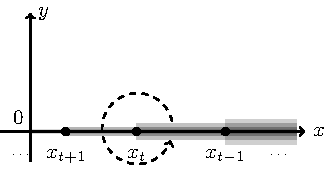
\includegraphics[width=0.5\linewidth]{img/complex-plane}
  \caption{%
    Fields are glued on the $x < 0$ semi-axis with non trivial discontinuities for $x_t < x < x_{t-1}$ for $t = 1,\, 2,\, \dots,\, N$ and where $x_t = \exp( \htau_{E,\, (t)} )$.
  }
  \label{fig:complex-plane}
\end{figure}

We consider a set of coordinates on the upper half \ccH of the complex plane:
\begin{equation}
  u = e^{\xi} \in \ccH,
\end{equation}
where $\xi = \tau_E + i \sigma$ and $\sigma \in \qty[ 0, \pi ]$ define the usual strip, and $\ccH = \qty{ w \in \C \mid \Im w \ge 0 }$.
These coordinates can then be extended to the entire complex plane by considering
\begin{equation}
  z = e^{\zeta} \in \C,
\end{equation}
where $\zeta = \tau_E + i \phi$ and $\phi \in \qty[0, 2\pi ]$ define the double strip.
Under this change of coordinates the Euclidean action~\eqref{eq:S_Eu_strip} becomes
\begin{equation}
  \begin{split}
    S_E
    & =
    \frac{T}{2}
    \iint \dd{u}\dd{\bu}\,
    \frac{1}{2}\,
    \qty(
      \frac{1}{u}\, \hpsi_{E,\, +,\, i}^* \lrpartial{\bu} \hpsi_{E,\, +}^i
      +
      \frac{1}{\bu}\, \hpsi_{E,\, -,\, i}^* \lrpartial{u} \hpsi_{E,\, -}^i
    )
    \\
    & =
    \frac{T}{2}
    \iint \dd{u}\dd{\bu}\,
    \frac{1}{2}\,
    \qty(
      \psi_{E,\, +,\, i}^* \lrpartial{\bu} \psi_{E,\, +}^i
      +
      \psi_{E,\, -,\, i}^* \lrpartial{u} \psi_{E,\, -}^i
    ),
  \end{split}
\end{equation}
where we introduce the off-shell field redefinitions:
\begin{equation}
  \psi_{E,\, +}^i(u,\, \bu)
  =
  \frac{1}{\sqrt{u}}\, \hpsi_{E,\, +}^i( \xi,\, \bxi ),
  \qquad
  \psi_{E,\, -}^i(u,\, \bu)
  =
  \frac{1}{\sqrt{\bu}}\, \hpsi_{E,\, -}^i( \xi,\, \bxi ).
  \label{eq:euclidean-off-shell-redefinitions}
\end{equation}
Fields with the hat sign on top thus represent strip and double strip definitions, while fields without the hat sign are defined on $\ccH$ or $\C$.\footnotemark{}
\footnotetext{%
  We could have anticipated these redefinitions from a CFT argument where
    \begin{equation*}
      \psi( u ) = \eval{\qty( \dv{u}{\xi} )^{-\frac{1}{2}}
        {\hpsi}(\xi)}_{\xi = \ln( u )},
    \end{equation*}
  but we cannot and do not rely on CFT properties since we have not shown that the theory is a CFT yet.
}
Notice that this is the result one would expect from the engineering dimension: in this case it works since the theory is essentially free.
Using the redefinitions~\eqref{eq:euclidean-off-shell-redefinitions}, the off-shell ``complex conjugation'' $\star$ then becomes
\begin{equation}
  \qty[ \psi_{E,\, +,\, i}( u,\, \bu ) ]^\star
  =
  \frac{1}{\bu}\, \psi_{E,\, +,\, i}^*\qty( \frac{1}{\bu},\, \frac{1}{u} ),
  \qquad
  \qty[ \psi_{E,\, -,\, i}( u,\, \bu ) ]^\star
  =
  \frac{1}{u}\, \psi_{E,\, -,\, i}^*\qty( \frac{1}{\bu},\, \frac{1}{u} ).
\end{equation}

We choose to insert the cut of the square root on the real negative axis.
The boundary conditions are then translated into
\begin{equation}
  \begin{cases}
    \psi_{E,\, -}^i( x - i\, 0^+ )
    =
    \tensor{\qty( R_{(t)} )}{^i_j} \psi_{E,\, +}^j( x + i\, 0^+ )
    \\
    \psi^{*}_{E,\, -,\, i}( x - i\, 0^+ ) =
    \tensor{\qty( R_{(t)}^* )}{_i^j} \psi^{*}_{E,\, +,\, j}( x + i\, 0^+ )
  \end{cases}
\end{equation}
for $x \in \qty( x_{(t)}, x_{(t-1)} )$, where $x_{(t)} = \exp( \htau_{E,\, (t)} ) > 0$, and
\begin{equation}
  \psi_{E,\, -}^i( x - i\, 0^+ )
  =
  \psi_{E,\, +}^i( x + i\, 0^+ ),
  \qquad
  \psi^{*}_{E,\, -,\, i}( x - i\, 0^+ )
  =
  \psi^{*}_{E,\, +,\, i}( x + i\, 0^+ )
\end{equation}
for $x<0$.

The product~\eqref{eq:euclidean-conserved-product-strip} is then
\begin{equation}
  \consprod{\alpha^*}{\beta}
  =
  -i \cN\,
  \qty[
    \int\limits_{\widehat{\Sigma}} \dd{u}
    \alpha^*_{+,\, i}(u) \beta_+^i(u)
    -
    \int\limits_{\widehat{\overline{\Sigma}}} \dd{\bu}
    \alpha^*_{-,\, i}(\bu) \beta_-^i(\bu)
  ],
  \label{eq:prod_H}
\end{equation}
where integrations are computed over two semi-circles $\widehat{\Sigma} = \qty{ u \in \C \mid \abs{u} = \exp( \htau_E ),\, 0 \le \Im u \le \pi }$ and $\widehat{\overline{\Sigma}} = \qty{ u \in \C \mid \abs{u} = \exp( \htau_E ),\, -\pi \le \Im u \le 0}$.
The stress-energy tensor becomes:\footnotemark{}
\footnotetext{%
  While rewriting the operator part of the stress-energy tensor from the strip
  formulation into the coordinates in $\ccH$ we actually get
  \begin{equation*}
    \cT_{\xi \xi}( \xi(u) ) = u^2\, \cT_{u u}( u ).
  \end{equation*}
  The reason of the presence of $u^2$ factor can be explained in two ways.
  Using GR we know that $\cT_{\xi \xi}( \xi ) \dss[2]{\xi} = \cT_{u u}( u ) \dss[2]{u}$.
  Another way is to notice that a translation in $\xi$ is a dilatation of $u$: the infinitesimal generator of $\xi$ translation must be the infinitesimal
  generator of $u$ dilatation, that is:
  \begin{equation*}
    P_{\xi}
    \sim
    \int \dd{\sigma}\, \cT_{\xi \xi}
    \sim
    D_u
    \sim 
    \int \dd{u}\, u\, \cT_{u u}.
  \end{equation*}
}
\begin{equation}
  \begin{split}
    \cT_{u u}( u )
    & =
    - \frac{\pi T}{2}\,
    \psi_{E,\, +,\, i}^*( u )\, \lrpartial{u} \psi^i_{E,\, +}( u )
    +
    \widehat{\cC}(u ),
    \\
    \cT_{\bu \bu}( \bu )
    & =
    - \frac{\pi T}{2}\,
    \psi_{E,\, -,\, i}^*( \bu )\, \lrpartial{\bu} \psi^i_{E,\, -}( \bu )
    +
    \widehat{\overline{\cC}}( \bu ).
  \end{split}
\end{equation}
Finally the anti-commutation relations are
\begin{equation}
  \begin{cases}
    \eval{
      \qty[
        \psi_{E,\, +}^i( u_1,\, \bu_1 )
        ,
        \psi_{E,\, +,\, j}^*( u_2,\, \bu_2 )
      ]_+
    }_{\abs{u_1} = \abs{u_2}}
    & =
    \frac{2}{T u_1}\, \tensor{\delta}{^i_j}\, \delta( \arg(u_1) - \arg(u_2) )
    \\
    \eval{
      \qty[
        \psi_{E,\, -}^i( u_1,\, \bu_1 )
        ,
        \psi_{E,\, -,\, j}^*( u_2,\, \bu_2 )
      ]_+
    }_{\abs{u_1} = \abs{u_2}}
    & =
    \frac{2}{T \bu_1}\, \tensor{\delta}{^i_j}\, \delta( \arg(u_1) - \arg(u_2) ),
  \end{cases}
\end{equation}
which despite the strange look of the expression are perfectly compatible with the definition~\eqref{eq:upper-half-extraction} leading to:
\begin{equation}
  \qty[ b_n,\, b^*_m ]_+
  =
  \frac{2 \cN}{T}\,
  \lconsprod{\dual{\hpsi}^*_{E,\, n}}{\dual{\hpsi}_{E,\, m}}
  =
  \frac{2 \cN}{T}\,
  \lconsprod{\dual{\psi}^*_{E,\, n}}{\dual{\psi}_{E,\, m}}
\end{equation}
when the product $\lconsprod{\cdot}{\cdot}$ is defined according to~\eqref{eq:prod_H}.
We expand the fields in modes as:
\begin{equation}
  \begin{cases}
    \psi^i_{E,\, +}(u)
    =
    \sum\limits_{n \in \Z} b_n\, \psi^i_{E,\, +,\, n}(u)
    \\
    \psi^i_{E,\, -}(\bu)
    =
    \sum\limits_{n \in \Z} b_n\, \psi^i_{E,\, -,\, n}(\bu)
  \end{cases}
\end{equation}
and
\begin{equation}
  \begin{cases}
    \psi^*_{E,\, +,\, i}(u)
    =
    \sum\limits_{n \in \Z} b^*_n\, \psi^*_{E,\, +,\, n,\, i}(u)
    \\
    \psi^*_{E,\, -,\, i}(\bu)
    =
    \sum\limits_{n \in \Z} b^*_n\, \psi^*_{E,\, -,\, n,\, i}(\bu)
  \end{cases}
\end{equation}
and $\dual{\psi}_{E,\, n}$ and $\dual{\psi}^*_{E,\, n}$ are the corresponding dual modes on the upper half plane.   


\subsection{Fields on the Complex Plane and the Doubling Trick}
  
We use again the doubling trick to define the fields on the subset $\C \setminus \qty[ x_{(N)},\, x_{(1)} ]$:
\begin{equation}
  \Psi( z )
  =
  \begin{cases}
    \psi_{E,\, +}(u)
    & \qfor
    z = u \in \ccH \setminus \qty[ x_{(N)}, x_{(1)} ]
    \\
    \psi_{E,\, -}(\bu)
    & \qfor
    z = \bu \in \overline{\ccH} \setminus \qty[ x_{(N)}, x_{(1)} ]
  \end{cases}
\end{equation}
where $z = \exp( \tau_E + i\, \phi ) = x + i y$ and $\overline{\ccH} = \qty{ w \in \C \mid \Im w \le 0 }$.
The same procedure applies also to $\Psi^*$ with the exchange $\psi_{E,\, \pm} \leftrightarrow \psi_{E,\, \pm}^*$.

In this case the ``complex conjugation'' $\star$ acts off-shell as
\begin{equation}
  \qty[ \Psi^i( z, \bz ) ]^\star
  =
  \frac{1}{\bz}\, \Psi_i^*\qty(\frac{1}{\bz}, \frac{1}{z}).
  \label{eq:complex-plane-conjugate}
\end{equation}
The boundary conditions then become:
\begin{equation}
  \begin{cases}
    \Psi^i( x - i\, 0^+ )
    & =
    \tensor{\qty( R_{(t)} )}{^i_j} \Psi^j( x + i\, 0^+ ),
    \\
    \Psi^{*\, i}( x - i 0^+ )
    & =
    \tensor{\qty( R_{(t)}^* )}{^i_j} \Psi^{*\, j}( x + i\, 0^+ ),
  \end{cases}
  \label{eq:boundary-condition-euclidean}
\end{equation}
for $x \in \qty( x_{(t)}, x_{(t-1)} )$, where $x_{(t)} = \exp( \htau_{E,\, (t)} ) > 0$ for $t \in \qty{ 1,\, 2,\, \dots,\, N }$.
When $x < 0$ we get
\begin{equation}
  \begin{cases}
    \Psi( x - i\, 0^+ ) & = \Psi( x + i\, 0^+ ),
    \\
    \Psi^*( x - i\, 0^+ ) & = \Psi^*( x + i\, 0^+ )
  \end{cases}.
  \label{eq:gluing-conditions-euclidean}
\end{equation}

Given the relations $\dd{z} = i\, z\, \dd{\phi}$, we can write the conserved product \eqref{eq:prod_H} as:
\begin{equation}
  \consprod{A^*}{B}
  =
  2\pi \cN
  \oint\limits_{\abs{z} = \exp( \tau_E )}
  \frac{\dd{z}}{2 \pi i}\, A^*_i( z )\, B^i( z ),
  \label{eq:conserved-product-complex-plane}
\end{equation}
where we explicitly stressed that the integral has to be performed at a fixed Euclidean time $\tau_E$: in the new coordinate on the plane the conserved product becomes a contour integral at a fixed radius from the origin.

In the same way we can recast the stress-energy tensor components~\eqref{eq:stress-energy-tensor-lightcone} in the new coordinates:
\begin{equation}
  \cT( z )
  =
  - \frac{\pi T}{2}\,
  \Psi^*_i( z )\, \lrpartial{z} \Psi^i( z )
  +
  \cC( z ),
\end{equation}
where $\cT = \cT_{zz}$ for simplicity.

Finally the canonical anti-commutation relations between the fields are:
\begin{equation}
  \eval{
    \qty[
      \Psi^i( z_1 ),\,
      \Psi_{j}^*( z_2 )
    ]_+
  }_{\abs{z_1} = \abs{z_2}}
  =
  \frac{2}{T z_1}\, \tensor{\delta}{^i_j}\, \delta( \arg(z_1) - \arg(z_2) ).
\end{equation}
The fields expansion in modes thus reads
\begin{equation}
  \Psi^i(z)
  =
  \sum\limits_{n \in \Z} b_n\, \Psi^i_{n}(z),
  \qquad
  \Psi^*_{i}(z)
  =
  \sum\limits_{n \in \Z} b^*_n\, \Psi^*_{n. i}(z).
  \label{eq:complex-plane-mode-expansion}
\end{equation}
The anti-commutation relations among the operators are
\begin{equation}
  \qty[ b_n,\, b^*_m ]_+
  =
  \frac{2 \cN}{T}\, \lconsprod{\dual{\Psi}^*_{n}}{\dual{\Psi}_{m}},
\end{equation}
when we introduce the dual modes
$\dual{\Psi}_{n}(z)$ and $\dual{\Psi}^*_{n}(z)$ whose normalization is
\begin{equation}
  \lconsprod{\dual{\Psi}^*_{n}}{{\Psi}_{m}}
  =
  \lconsprod{\dual{\Psi}_{n}}{{\Psi}^*_{m}}
  =
  \delta_{m,n}.
\end{equation}


\subsection{Algebra of Creation and Annihilation Operators}
\label{sec:modes_and_algebra}
  
In this section we find the explicit expression of the modes which satisfy the \eom and the boundary conditions.
We then compute the dual fields and finally the algebra of the creators and annihilators.


\subsubsection{NS Complex Fermions}
\label{sec:ns-complex-fermions}

We start from NS complex fermions to show that the formalism can recover known results.
Consider the usual definition:
\begin{equation}
  \begin{cases}
    \psi_-^i( \tau, 0 )
    & =
    \psi_+^i( \tau, 0 ),
    \\
    \psi_-^i( \tau, \pi )
    & =
    -\psi_+^i( \tau, \pi )
  \end{cases}
\end{equation}
for $\tau \in \R$, which can be recovered from~$\eqref{eq:boundary-conditions-solutions}$ setting $R_{(t)} \equiv \1$.
In the Euclidean formulation we use~\eqref{eq:boundary-condition-euclidean} and~\eqref{eq:gluing-conditions-euclidean} to get:
\begin{equation}
  \begin{cases}
    \Psi( x - i\, 0^+ ) & =  \Psi( x + i\, 0^+ )
    \\
    \Psi^*( x - i\, 0^+ ) & =  \Psi^*( x + i\, 0^+ )
  \end{cases}
\end{equation}
for $x \in \R$.

We define:
\begin{eqnarray}
  \Psi^i_{( n,\, i_0 )}( z )
  & = &
  \cN_{\Psi}\, \delta^i_{i_0}\, z^{-n},
  \\
  \dual{\Psi}_{( m,\, j_0 ),\, j}( z )
  & = &
  \qty( 2 \pi \cN\, \cN_{\Psi} )^{-1}\, \delta_{j, j_0}\, z^{m-1}
\end{eqnarray}
to recover the definition of the dual modes~\eqref{eq:conserved-product-dual-basis} using the Euclidean conserved product \eqref{eq:conserved-product-complex-plane}.
We then proceed similarly for $\Psi^*$ in such a way that
\begin{equation}
  \lconsprod{\dual{\Psi}_{( n,\, i_0 )}^*}{\Psi_{( m,\, j_0 )}}
  =
  \lconsprod{\dual{\Psi}_{( m,\, j_0 )}}{\Psi^*_{( n,\, i_0 )}}
  =
  \delta_{n, m}\, \delta_{i_0, j_0}.
\end{equation}
As a consequence we find
\begin{equation}
  \lconsprod{\dual{\Psi}_{( n,\, i_0 )}^*}{\dual{\Psi}_{( m,\, i_1 )}}
  =
  \frac{1}{2 \pi \cN\, \cN^2_{\Psi}}\, \delta_{i_0, i_1}\, \delta_{n + m, 1}.
\end{equation}

Consider the  NS expansion in modes of the double fields:
\begin{eqnarray}
  \Psi^i( z )
  & = &
  \sum\limits_{n \in \Z}\,
  \sum\limits_{i_0}\,
  b_{(n,\, i_0)}\, \Psi^i_{( n,\, i_0 )}( z ),
  \\
  \Psi^{*}_i( z )
  & = &
  \sum\limits_{n \in \Z}\,
  \sum\limits_{i_0}\,
  b^*_{(n,\, i_0)}\, \Psi^{*}_{( n,\, i_0 ),\, i}( z ),
\end{eqnarray}
then
\begin{eqnarray}
  b_{( n,\, i_0 )}
  & = &
  \lconsprod{\dual{\Psi}_{( n,\, i_0 )}^*}{\Psi},
  \\
  b^*_{( n,\, i_0 )}
  & = &
  \lconsprod{\dual{\Psi}_{( n,\, i_0)}}{\Psi^*},
\end{eqnarray}
and
\begin{equation}
  \qty[ b_{( n, i_0 )},\, b^*_{( m, j_0 )} ]_+
  =
  \frac{1}{\pi T \cN_{\Psi}^2}\, \delta_{i_0, j_0}\, \delta_{n + m, 1}.
  \label{eq:ns-algebra}
\end{equation}


% vim: ft=tex
